% Options for packages loaded elsewhere
\PassOptionsToPackage{unicode}{hyperref}
\PassOptionsToPackage{hyphens}{url}
%
\documentclass[
]{book}
\usepackage{amsmath,amssymb}
\usepackage{iftex}
\ifPDFTeX
  \usepackage[T1]{fontenc}
  \usepackage[utf8]{inputenc}
  \usepackage{textcomp} % provide euro and other symbols
\else % if luatex or xetex
  \usepackage{unicode-math} % this also loads fontspec
  \defaultfontfeatures{Scale=MatchLowercase}
  \defaultfontfeatures[\rmfamily]{Ligatures=TeX,Scale=1}
\fi
\usepackage{lmodern}
\ifPDFTeX\else
  % xetex/luatex font selection
\fi
% Use upquote if available, for straight quotes in verbatim environments
\IfFileExists{upquote.sty}{\usepackage{upquote}}{}
\IfFileExists{microtype.sty}{% use microtype if available
  \usepackage[]{microtype}
  \UseMicrotypeSet[protrusion]{basicmath} % disable protrusion for tt fonts
}{}
\makeatletter
\@ifundefined{KOMAClassName}{% if non-KOMA class
  \IfFileExists{parskip.sty}{%
    \usepackage{parskip}
  }{% else
    \setlength{\parindent}{0pt}
    \setlength{\parskip}{6pt plus 2pt minus 1pt}}
}{% if KOMA class
  \KOMAoptions{parskip=half}}
\makeatother
\usepackage{xcolor}
\usepackage{longtable,booktabs,array}
\usepackage{calc} % for calculating minipage widths
% Correct order of tables after \paragraph or \subparagraph
\usepackage{etoolbox}
\makeatletter
\patchcmd\longtable{\par}{\if@noskipsec\mbox{}\fi\par}{}{}
\makeatother
% Allow footnotes in longtable head/foot
\IfFileExists{footnotehyper.sty}{\usepackage{footnotehyper}}{\usepackage{footnote}}
\makesavenoteenv{longtable}
\usepackage{graphicx}
\makeatletter
\def\maxwidth{\ifdim\Gin@nat@width>\linewidth\linewidth\else\Gin@nat@width\fi}
\def\maxheight{\ifdim\Gin@nat@height>\textheight\textheight\else\Gin@nat@height\fi}
\makeatother
% Scale images if necessary, so that they will not overflow the page
% margins by default, and it is still possible to overwrite the defaults
% using explicit options in \includegraphics[width, height, ...]{}
\setkeys{Gin}{width=\maxwidth,height=\maxheight,keepaspectratio}
% Set default figure placement to htbp
\makeatletter
\def\fps@figure{htbp}
\makeatother
\setlength{\emergencystretch}{3em} % prevent overfull lines
\providecommand{\tightlist}{%
  \setlength{\itemsep}{0pt}\setlength{\parskip}{0pt}}
\setcounter{secnumdepth}{5}
\usepackage{booktabs}
\ifLuaTeX
  \usepackage{selnolig}  % disable illegal ligatures
\fi
\usepackage[]{natbib}
\bibliographystyle{plainnat}
\usepackage{bookmark}
\IfFileExists{xurl.sty}{\usepackage{xurl}}{} % add URL line breaks if available
\urlstyle{same}
\hypersetup{
  pdftitle={Material Básico GCADMO},
  pdfauthor={Hugo Sasaki, Julyana Alvez e Luiz Garutti},
  hidelinks,
  pdfcreator={LaTeX via pandoc}}

\title{Material Básico GCADMO}
\author{Hugo Sasaki, Julyana Alvez e Luiz Garutti}
\date{2025-08-25}

\begin{document}
\maketitle

{
\setcounter{tocdepth}{1}
\tableofcontents
}
\chapter*{Sobre o Livro}\label{sobre-o-livro}
\addcontentsline{toc}{chapter}{Sobre o Livro}

Este pequeno livro feito pelos alunos do GCADMO apresenta alguns materiais e aulas com alguns conteúdos base tanto para aqueles que desejam entrar, ou que já fazem parte do grupo.

Entretanto, o campo da Pesquisa Operacional é bastante amplo, e o livro ainda está em processo de desenvolvimento, por isso pode não conter todos os materiais que deseja no presente momento, mas saiba que um dia chegaremos lá!

Considerando isso, o livro já conta com uma lista de exercícios de modelação retirado de outros livros relevantes no campo da Pesquisa Operacional que o usuário pode tentar resolver.

\chapter*{Introdução a Python}\label{introduuxe7uxe3o-a-python}
\addcontentsline{toc}{chapter}{Introdução a Python}

Capítulo sobre os básicos da linguagem usada em python pedir pro Luiz ou pra Julyana elaborar

\chapter*{Exercícios}\label{exercuxedcios}
\addcontentsline{toc}{chapter}{Exercícios}

\begin{center}\rule{0.5\linewidth}{0.5pt}\end{center}

\section*{Exercício 1}\label{exercuxedcio-1}
\addcontentsline{toc}{section}{Exercício 1}

\textbf{(Katta Murty 1.26)} Uma agência controla a operação de um sistema que consiste em dois reservatórios de água com uma usina hidrelétrica acoplada a cada um. O horizonte de planejamento para o sistema é de um ano, dividido em seis períodos. O reservatório 1 tem capacidade para armazenar 3500 kilo acres-pés de água e o reservatório 2 tem capacidade para 5500 kilo acres-pés. Em qualquer instante de tempo, se o reservatório estiver em sua capacidade máxima, a água adicional que entrar será descartada por meio de um vertedouro. A água descartada não produz eletricidade.

Durante cada período, uma quantidade mínima especificada de água deve ser liberada dos reservatórios para atender às necessidades a jusante de recreação, irrigação e navegação. Entretanto, não há limite superior para a quantidade de água que pode ser liberada dos reservatórios. Qualquer água não liberada é armazenada (até a capacidade do reservatório) e pode ser utilizada para liberação em períodos subsequentes. Toda a água liberada dos reservatórios (mesmo que seja liberada para recreação e outros propósitos) produz eletricidade.

Pode-se assumir que, durante cada período, as entradas e liberações de água ocorrem a uma taxa constante. Além disso, em média, 1 acre-pé de água liberada do reservatório 1 produz 310 kWh de eletricidade, e 1 acre-pé liberado do reservatório 2 produz 420 kWh.

No início do ano, o reservatório 1 contém 1800 kilo acres-pés de água e o reservatório 2 contém 2500 kilo acres-pés de água. As mesmas quantidades de água devem permanecer nos respectivos reservatórios no final do ano.

A eletricidade produzida pode ser vendida a um consumidor local (chamado de cliente classe I) ou a clientes classe II.

Um cliente classe I compra eletricidade com base anual; ele exige que porcentagens especificadas dela sejam fornecidas em vários períodos. Ele paga \$10,00/1000 kWh.

Um cliente classe II compra eletricidade período a período. Ele comprará qualquer quantidade de eletricidade em qualquer período a \$5,00/1000 kWh.

Os dados do problema são apresentados a seguir.

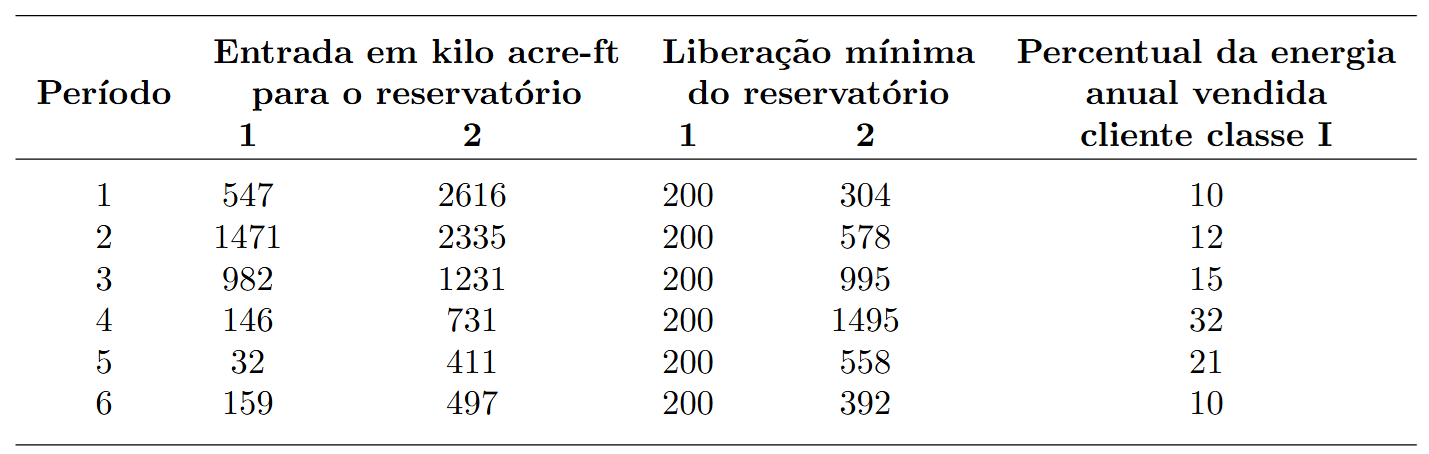
\includegraphics{Imagens/TabelaEx_1.png}

Opere o sistema para maximizar o lucro anual total da venda de eletricidade.

\begin{center}\rule{0.5\linewidth}{0.5pt}\end{center}

\section*{Exercício 2}\label{exercuxedcio-2}
\addcontentsline{toc}{section}{Exercício 2}

\textbf{(Katta Murty 1.23)} Uma empresa europeia possui três plantas de coquerias (fornos de coque), codificadas como 1, 2 e 3. O carvão vem de quatro fontes diferentes: EUA, Ruhr, Lorena e Sarre. As plantas produzem coque, que pode ser classificado em duas categorias: coque metalúrgico, que é o mais valorizado e usado na produção de aço e os chamados ``finos de coque'', que são pedaços pequenos ou pó resultante do processo; elas também produzem gás de forno de coque.

As plantas de coquerias são operadas aquecendo-as com gás de alto-forno ou gás de coqueria. O fluxograma do processo é apresentado na figura a seguir. A produção de gás de coqueria e de coque depende do carvão utilizado.

*\textbf{A quantidade de gás de forno de coque produzida é medida pelo seu conteúdo energético. Kth é uma kilothermie, onde thermie é a quantidade de calor necessária para elevar a temperatura de 1 tonelada de água em 1 grau Celsius.}**Tonelada

A proporção de finos de coque no coque produzido depende do carvão usado e da planta onde ele é utilizado.

O coque metalúrgico é o que sobra no coque após a separação dos finos de coque.

Processar uma tonelada de carvão requer o equivalente energético a 0,611 Kth de gás de forno de coque. Uma unidade de gás de alto-forno equivale a 0,927 Kth de gás de forno de coque.

As capacidades anuais de processamento das três plantas são de 9 × 105 tonelada, 7 × 105 toneladas e 3 × 105 toneladas de carvão, respectivamente.

O carvão de Saar não pode ser usado nas plantas 1 e 2. O carvão dos USA e Lorraine não podem ser usados na planta 3. A porcentagem do carvão de Lorraine usado na planta 1 não pode exceder 30. A porcentagem do carvão de Lorraine usado na planta 2 não pode exceder 35. A porcentagem do carvão de Saar usado na planta 3 não pode exceder 40.

Gás de coqueria pode ser comprado ou vendido em qualquer quantidade por \$11/Kth. Finos de coque podem ser vendidos em qualquer quantidade por \$98/tonelada. Gás de alto-forno pode ser comprado em qualquer quantidade por \$8/unit. O preços dos carvões são apresentados a seguir:

Todo o fino de coque produzido é vendido. Todo o gás de coqueria produzido é utilizado nas plantas ou vendido.

É necessário produzir um total de 106 toneladas de coque metalúrgico ao final do ano.

\begin{center}\rule{0.5\linewidth}{0.5pt}\end{center}

\section*{Exercício 3}\label{exercuxedcio-3}
\addcontentsline{toc}{section}{Exercício 3}

\textbf{(Caso BRF)} Uma empresa alimentícia aluga veículos para realizar as suas entregas. O setor de PCP junto ao departamento de logística faz o dimensionamento de toda carga que deve ser alocada a cada veículo, bem como a sua rota. Dessa forma, sabe-se, para cada dia de um horizonte de planejamento, quantos veículos serão necessesários. Esse dado é mostrado pela Tabela a seguir:

Cada contrato por um veículo permite que o mesmo seja utilizado por uma quantidade limitada de dias no horizonte de planejamento, e existe um custo associado ao contrato. O custo do contrato independe do número de dias que o veículo é alocado pela empresa. A próxima tabela mostra os tipos de contrato existentes:

a) Determine o modelo de PI para o problema de contratação e alocação de frota da BRF.
b) Escreva o modelo genérico (conjuntos, parâmetros, variáveis) para o problema.

\chapter*{Gabarito}\label{gabarito}
\addcontentsline{toc}{chapter}{Gabarito}

\phantomsection\label{conteudo-secreto}
\section*{Exercício 1}\label{exercuxedcio-1-1}
\addcontentsline{toc}{section}{Exercício 1}

\begin{center}\rule{0.5\linewidth}{0.5pt}\end{center}

\section*{Exercício 2}\label{exercuxedcio-2-1}
\addcontentsline{toc}{section}{Exercício 2}

\phantomsection\label{senha-div}
Digite a senha para acessar o gabarito:

Entrar

  \bibliography{book.bib,packages.bib}

\end{document}
